%
% galilei.tex -- schematische Darstellung der Galilei-Transformtion
%
% (c) 2017 Prof Dr Andreas Müller, Hochschule Rapperswil
%
\documentclass[tikz]{standalone}
\usepackage{times}
\usepackage{txfonts}
\usepackage{fp}
\usepackage{ifthen}
\usepackage[utf8]{inputenc}
\usetikzlibrary{arrows,intersections}
\usetikzlibrary{fixedpointarithmetic}
\begin{document}
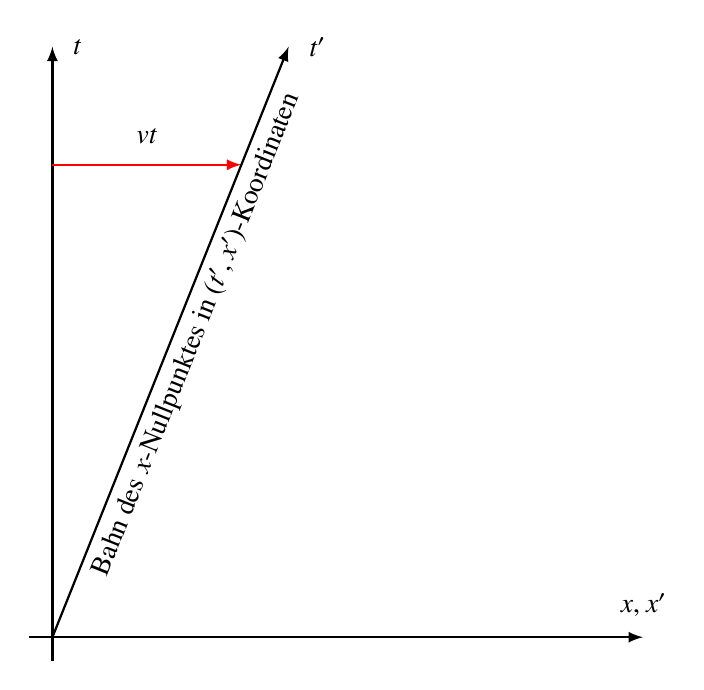
\begin{tikzpicture}[>=latex, thick, scale=1.5]

\draw[->] (-0.2,0)--(5,0);
\node[label={above:$x, x'$}] at (5,0) {};
\draw[->] (0,-0.2)--(0,5);
\node[label={right:$t$}] at (0,5) {};

\draw[->,red] (0,4)--(8/5,4);
\node[red,label={above:$vt$}] at (4/5,4) {};

\draw[->] (0,0)--(2,5);
\node[label={right:$t'$}] at (2,5) {};

\node[label={[rotate=atan(5/2)] Bahn des $x$-Nullpunktes in $(t',x')$-Koordinaten}] at (1.4,2.4) {};

\end{tikzpicture}
\end{document}
